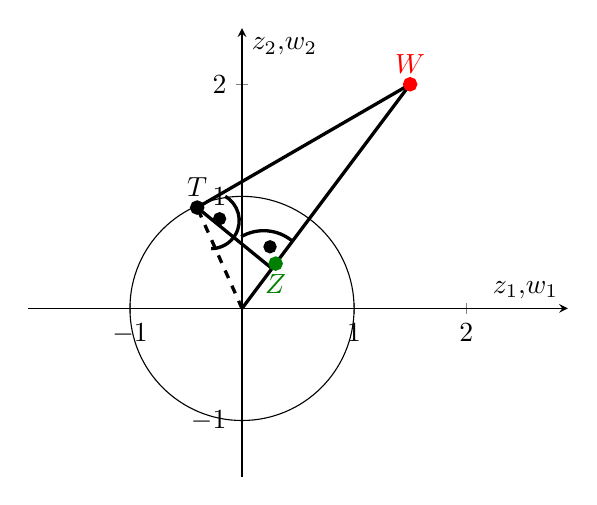
\begin{tikzpicture}
	\begin{axis}[
		axis lines=middle,
		axis equal,
		xmin=-0.5,
		xmax=1.5,
		ymin=-1.5,
		ymax=2.5,
		xlabel=$z_1\text{,} w_1$,
		ylabel=$z_2\text{,} w_2$,
		disabledatascaling
	]	
		\draw (axis cs: 0, 0) circle [radius=1];
		\addplot[-, very thick] coordinates {(0, 0) (1.5, 2)};
		\addplot[-, very thick] coordinates {(0.275, 0.35) (-0.4, 0.9)};
		\addplot[-, very thick] coordinates {(-0.4, 0.9) (1.5, 2)};
		\addplot[-, very thick, dashed] coordinates {(0, 0) (-0.4, 0.9)};
		\addplot[mark=*, very thick] coordinates {(-0.4, 0.9)} node[above] {$T$};
		\addplot[mark=*, very thick, black!50!green] coordinates {(0.3, 0.4)} node[below, black!50!green] {$Z$};
		\addplot[mark=*, very thick, red] coordinates {(1.5, 2)} node[above, red] {$W$};
		\draw [-, very thick] (axis cs:0.45, 0.6) arc [radius=0.4, start angle=50, end angle=120];
		\addplot[mark=*, thick] coordinates {(0.25, 0.55)};
		\draw [-, very thick] (axis cs:-0.15, 1) arc [radius=0.25, start angle=60, end angle=-90];
		\addplot[mark=*, thick] coordinates {(-0.2, 0.8)};
	\end{axis}
\end{tikzpicture}